\usetikzlibrary{positioning,matrix, arrows.meta}
\usetikzlibrary{shapes,arrows}

\tikzstyle{block} = [draw, rectangle, 
    minimum height=3em, minimum width=6em,fill=blue!30]
\tikzstyle{circ} = [draw, circle, node distance=1cm,fill=red!30]
\tikzstyle{input} = [coordinate]
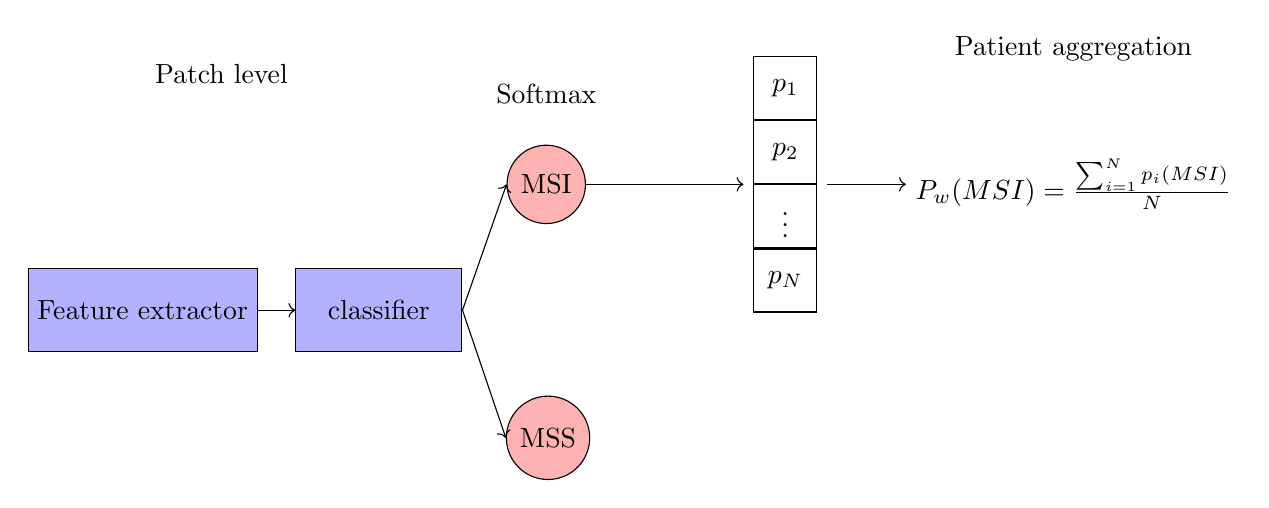
\begin{tikzpicture}
\node [input, name=input] {};
\node [block] (inception) at (0,0) {Feature extractor};
\node [block] (mlp) at (3,0) {classifier};
\node(D) at(1,3) {Patch level};
\node [circ, above right=of mlp] (msi) {MSI};
\node(C) [above=0.4cm of msi]{Softmax};
\node [circ, below right=of mlp] (mss) {MSS};
\matrix (A) [matrix of nodes, right=2cm of msi, nodes={draw, minimum size=8mm},column sep=-\pgflinewidth]
{    $p_1$\\$p_2$\\\vdots\\$p_N$\\};
\node(B)[right=of A]{
    \(P_w(MSI) = \frac{\sum_{i=1}^{N}p_i(MSI)}{N}\)};
\node(C) [above=of B]{Patient aggregation};
\draw [->] (inception.east) -- (mlp.west);
\draw [->] (mlp.east) -- (msi.west);
\draw [->] (mlp.east) -- (mss.west);
\draw [->] (msi.east) -- (A.west);
\draw[->] (A.east) -- (B.west);
\end{tikzpicture}
